\documentclass{article}
\usepackage[dvipsnames]{xcolor}
\usepackage{amsmath}
\usepackage{pgfplots}
\usepackage{graphicx}
\usepackage{enumitem}
\usepackage{centernot}
\usepackage{setspace}
\usepackage[margin=0.95in]{geometry}
\usepackage{titling}
\usepackage{tcolorbox}

\setlength{\droptitle}{-7em}   % This is your set screw

\begin{document}

\title{Philosophy of Physics\\Final Exam}
\author{Ozaner Hansha}
\date{May 8, 2020}
\maketitle
\setstretch{1.3}

\subsection*{Question 2}
\noindent\textbf{Prompt:} In what way does ordinary classical statistical mechanics (the Newtonian dynamical law plus the statistical postulate) fail to account for the asymmetry of thermodynamics? Use an example of a particular system, such as a partly melted ice cube in a glass of water, to illustrate the problem. Then explain how the Past Hypothesis is supposed to solve this problem.
\bigskip

\noindent\textbf{Response:} Consider a macrostate of the ice-glass-environment system, i.e. the average temperature of the components, pressure, etc. There are a whole continuum of microstates compatible with this macrostate. It can be shown that the vast majority, in a somewhat reasonable measure-theoretic sense, of these microstates tend towards a macrostate with a higher overall entropy. Equipped with the statistical postulate (which states that our system's particular microstate is uniformly likely to be any one of the compatible microstates), this implies that our system is highly likely to increase in entropy. This in turn corresponds to the temperature of the system becoming more diffuse and the ice melting, as we'd expect.

While this line of reasoning accurately describes our experience and observation that entropy increases over time, it leads us to a problem. Classical statistical mechanics (that is Newtownian mechanics and the statistical postulate) is time reversible, implying that our reasoning above is also time reversable. This is all to say that under SM as it is now, systems in the past are \textit{also} predicted to have their entropy increase. This is clearly counter to our observation which suggest that entropy was lower in the past and has increased over time. In terms of the ice cube, we usually predict that it was larger in the past and not that it was smaller and just happened to flucate into being the larger size it is now.

Albert accounts for this asymmetry via the past hypothesis (PH). Essentially, we posit that the initial state of the universe (or at least a state far enough before our observational capacity) was in a state of low entropy. This allows us to rid ourselves of the, all things being equal, much more likely possibility that the past had a higher entropy that the statistical postulate implies. We can phrase this more intuitively with conditional probabilities:
\begin{align*}
  P(\text{ice cube was larger in the past}) &\ll P(\text{ice cube was smaller in the past})\\
  P(\text{ice cube was larger in the past }|\text{ PH}) &\gg P(\text{ice cube was smaller in the past }|\text{ PH})
\end{align*}

Given the universe was originally in such a low entropy state, the increase of entropy over time \textit{and} the decrease backwards in time becomes the most probable outcome, matching up with what we observe.
The reasoning for the former is unchanged, but that entropy decreases backwards in time is a product of us taking to be true the low entropy initial state and that it is more likely that that state evolved gradually towards higher entropy rather than jumping up and down.

\subsection*{Question 3}
\noindent\textbf{Prompt:} Explain one of Carroll’s two main objections to the Past Hypothesis account of thermodynamics (either the objection based on the nature of the initial macrostate, or the one based on the idea of Boltzmann brains). How does Carroll’s own account claim to avoid the objection.
\bigskip

\noindent\textbf{Response:} Carroll considers our universe, one that we can reasonably assert satisfies the past hypothesis, in the form of the big bang, and also can be modeled as a de Sitter space. Such a universe will, bar any other conditions, eventually tend towards a thermal equilibrium and stay there for essentially all time after. Then, for any particular observer that could arise in the history of this universe consistent with our experience, in my case as a person typing a report on a computer, it is far more likely that they are a random fluctuation of lower entropy that occurred some arbitrary amount of time after thermal equilibrium rather than an actual human being who exists on the initial upswing of entropy after the big bang, a period of time much smaller than that of after the equilibrium:
\begin{align*}
  \text{big bang}&\rightarrow \text{galaxies form}\rightarrow \text{earth forms}\rightarrow\text{evolution}\rightarrow\cdots\rightarrow\underbrace{\text{me typing}}_{\text{less likely}}\tag{near big bang}\\
  \text{big bang}&\rightarrow\cdots\rightarrow\cdots\rightarrow\text{equilibrium}\rightarrow\cdots\rightarrow\cdots\rightarrow\underbrace{\text{me typing (fluctuation)}}_{\text{much more likely}}\tag{after equilibrium}
\end{align*} 
% $$\text{big bang}\rightarrow\cdots\rightarrow\cdots\rightarrow\text{equilibrium}\rightarrow\cdots\rightarrow\text{me typing (fluctuation)}$$ 

Moreover, it is by far most likely that this fluctuation represents the minimum physical system that is consistent with our experience, meaning it is far more likely for that fluctuation to be a floating disembodied brain that exists only for the period of time the experience requires.

Why is this a problem for the past hypothesis? Indeed, this objection poses a problem to \textit{any} physical theory or account that both allows for these so called \textbf{Boltzmann brains} as well as posits that they are the most likely explanation of our experience. This is because our entire understanding of whatever theory we initally posited came from the underlying assumption that our evidence, thoughts, and experience came from observing and thinking about the universe around us. But if that same theory predicts that it is more likely that all those thoughts, experience, and evidence are just products of a random fluctuation, a random fluctuation that could have equally produced bogus thoughts, experience, and evidence, how can we trust that theory in the first place? Such a theory would quite literally predict that it is most certainly wrong! Carroll aptly calls this situation \textbf{cognitively unstable}.

So, how do we avoid it? Well we can simply take the PH to be a law of the universe, just like we do its usual quantum dynamics. And, more precisely, we take the \textbf{near past hypothesis} (NPH) to be a law, which states that not only was there a low entropy initial state of the universe but that we exist on the initial upswing of entropy from this state. This solves the problem of Boltzmann brains but, as Carroll notes, it is not very satisfying. There is no explanation, it simply ``asserts'' the problem away.

In response to this, Carroll puts forth his own account of the past hypothesis (really \textit{near} past hypothesis) in the form of a speculative multiversal account of the birth of the universe. Essentially Carroll notes that it is plausible, up to a theory of quantum gravity, that a de Sitter space in thermal equilibrium, like the one we considered previously, could itself fluctuate, like any other quantum field, into a higher energy `plateau' often referred to as a \textbf{false vacuum}. After this extremely unlikely transition, it is even less likely that, instead of returning back to the true vacuum state of the surronding space, that fluctuation breaks off into what is called a \textbf{baby universe}, now totally disconnected from its parent universe. Since it was created from a false vacuum, this new baby universe has a high energy density (and so can create all the particles and energy we find in our universe) and inversely has a low entropy, satisfying the PH.

While the implication that our universe was once one of these baby universes explains the PH, it doesn't explain the NPH and thus we still are left to deal with Boltzmann brains. As Carroll notes however, this picture \textit{does} allows for an explanation of the NPH. In particular, if the rate of baby universes `spawning' in the multiverse is larger than that of the rate Boltzmann brains appear in the multiverse (mostly in universes that have reached equilibrium), then it is more likely that we are real (i.e. not Boltzmann brains) than not:
$$P(\substack{\text{baby universe with humans}\\\text{forms in the multiverse}})\gg P(\substack{\text{a Boltzmann brain}\\\text{forms in the multiverse}})\implies\underbrace{P(\text{\small We are `real' humans})\gg P(\text{\small We are Boltzmann brains})}_{\text{essentially a probablistic NPH}}$$

This is a huge if (on top of the other huge ifs like baby universes) but it can, possibly, be made more palatable by considering that if the laws of physics are slightly perturbed in every new baby universe (say via the fundamental physical constants taking on new similar but different values) then a process of universal evolution would take place. More precisely, we would find that the universes with constants more likely to spawn more baby universes would dominate the multiverse, thus further increasing the rate of baby universes spawning in a feedback loop akin to natural selection.

\subsection*{Question 4}
\noindent\textbf{Prompt:} What is the wave asymmetry? Give an example to illustrate it. How might the Past Hypothesis be able to account for this asymmetry?
\bigskip

\noindent\textbf{Response:} Whenever we observe a wave we always see it spreading out \textit{after} its source is excited. This is innocuous at first, almost obvious, but considering that the laws of physics (in this case the wave equation) are TRI, we should equally be able to see the time reverse of such a wave. Such a wave would initially be spread out and then converge towards some source, rather than emanate from that source.

Put more formally, we call a solution to the wave equation a wave. Solutions where the wave's motion appears after the source accelerates are called \textbf{retarded} solutions, while solutions where the wave's motion precedes the source's acceleration are called \textbf{advanced} solutions.

To make this more explicit, consider a pebble thrown into a pond. From the point on the surface the pebble touched (i.e. the source) a wave of water will emanate outwards. This is a retarded wave. Now consider the time reverse of this. There would be a wave on the pond set up in such a way as to have it converge at the source with the same intensity that dropping the pebble caused. This is an advanced wave.

At first blush, this is the wave asymmetry. That nature only seems to demonstrate retarded waves and not advanced ones, despite both being valid solutions to the wave equation. However, when we consider that there is a underlying background field, or \textbf{free field}, and not just the retarded/advanced field we have been considering, things can become a bit more complicated.

Before we continue, let us make clear what such a field could look like. Consider a charge producing an EM wave due to being accelerated. The retarded/advanced field here is just the regular EM field while the free field here is something like the CMB. The CMB, of course, exists on the EM field but we can separate the CMB component and the component wave the charge produces from the total observed wave. With that example in mind, consider the following scenarios. On the left is what we usually take to happen when, say, a charge emits an EM wave. On the right, however, we have an advanced wave converging on the charge. We might describe the charge as emitting an EM wave to the \textit{past} in this scenario:
\newline 
\pgfplotsset{%
    compat=newest, %footnotesize
    tick label style={font=\footnotesize},
    label style={font=\small},
    legend style={font=\small},
    axis x line = center,
    axis y line = center,
    every axis/.style={pin distance=1ex},
    trim axis left}

\begin{center}
\begin{tcolorbox}[width=.475\textwidth, nobeforeafter, title=Retarded Solution]
\begin{tikzpicture}
\begin{axis}[
  axis x line=center,
  ymin=-5,ymax=5,
  axis y line=none,
  xmin=-6*pi,xmax=6*pi,
  xticklabels={,,} 
  ]
  \addplot[domain=0:6*pi,blue]{.15};
  \addlegendentry{Free Field}
  \addplot[domain=0:6*pi,samples=200,red]{sin(deg(x))-.2};
  \addlegendentry{Retarded Field}
  \addplot[domain=0:6*pi,samples=200,cyan]{sin(deg(x))};
  \addlegendentry{Total Field}
  \node[circle,fill,scale=.5] at (axis cs:0,0) {};
  \node[circle] at (axis cs:0,1.4) {source};
  \node[circle] at (axis cs:-6*pi+3,1.4) {past};
  \node[circle] at (axis cs:6*pi-3,1.4) {future};
  \addplot[domain=-6*pi:0,blue]{.15};
  \addplot[domain=-6*pi:0,red]{-.15};
  \addplot[domain=-6*pi:0,cyan]{0};
\end{axis}
\end{tikzpicture}
\end{tcolorbox}\hfill
\begin{tcolorbox}[width=.475\textwidth, nobeforeafter, title=Advanced Solution]
\begin{tikzpicture}
\begin{axis}[
  axis x line=center,
  ymin=-5,ymax=5,
  axis y line=none,
  xmin=-6*pi,xmax=6*pi,
  xticklabels={,,}
  ]
  \addplot[domain=-6*pi:6*pi,samples=200,blue]{sin(deg(x))-.2};
  \addlegendentry{Free Field}
  \addplot[domain=0:6*pi,red]{.15};
  \addlegendentry{Advanced Field}
  \addplot[domain=0:6*pi,samples=200,cyan]{sin(deg(x))};
  \addlegendentry{Total Field}
  \node[circle,fill,scale=.2] at (axis cs:0,0) {};
  \node[circle] at (axis cs:0,1.4) {source};
  \node[circle,fill,scale=.5] at (axis cs:0,0) {};
  \node[circle] at (axis cs:-6*pi+3,1.4) {past};
  \node[circle] at (axis cs:6*pi-3,1.4) {future};
  \addplot[domain=-6*pi:0,samples=200,red]{sin(deg(x+3*pi))-.2};
  \addplot[domain=-6*pi:0,cyan]{0};
\end{axis}
\end{tikzpicture}
\end{tcolorbox}
\end{center}

\textit{*Note that the component waves are a little offset for ease of visibility.}
\newline

The problem we are now faced with is that, while the right scenario seems preposterous (or at least very unlikely), both situations produce the same total wave and thus net the same observation. We seem to be in a situation analogous to that of the thermodynamic asymmetry. As such, it might seem promosing to take a similar stance and simply declare that only retarded solutions to the wave equation are valid, a ``retardation condition,'' just as we asserted the past hypothesis. However, there is a better solution. In particular, we can use the PH to show that retarded waves are far more likely than advanced ones. Doing this would allow us to kill two birds (wave and thermodynamic asymmetry) with one stone (the PH) and thus may be a more desirable solution.

So, how does the PH do it? Well starting with the big bang, which of course satisfies the PH, we have the following chain of reasoning:

% \begin{gather*}
%   \underbrace{\overbrace{\text{Big Bang}}^{\text{Thermal equilibrium}}}_{\substack{\text{Dense, uniformly hot state}\\\text{Gravitational entropy }\downarrow\\\text{Thermal entropy }\uparrow}}\implies
%   \underbrace{\overbrace{\text{Large masses form}}^{\text{Thermal disequilibrium}}}_{\substack{\text{Clumps of dense hot matter}\\\text{Gravitational entropy }\uparrow\\\text{Thermal entropy }\downarrow}}\\
%   \implies P(\substack{\text{accelerating charges in dense}\\\text{clumps will emit waves to future }}|\substack{\text{thermal}\\\text{ disequilibrium}})\gg
%   P(\substack{\text{accelerating charges in dense}\\\text{clumps will emit waves to past }}|\substack{\text{thermal}\\\text{ disequilibrium}})
% \end{gather*}

\begin{align*}
  \overbrace{\text{Big Bang}}^{\substack{\text{Dense, uniformly hot state}\\\rightarrow\text{ Thermal equilibrium}}}
  &\implies\overbrace{\text{Stars form}}^{\substack{\text{Clumps of dense hot matter}\\\rightarrow\text{ Thermal disequilibrium}}}\\
  &\implies P\left(\substack{\text{accelerating charges}\\\text{in dense clumps will }\\\text{emit waves to future}}|\substack{\text{thermal}\\\text{ disequilibrium}}\right)\gg
  P\left(\substack{\text{accelerating charges}\\\text{in dense clumps will }\\\text{emit waves to past}}|\substack{\text{thermal}\\\text{ disequilibrium}}\right)
\end{align*}

Put in a less cryptic way, the initially low entropy (but high thermal entropy) big bang state eventually evolves into a universe with large clumps of hot dense matter (e.g. stars) and empty space in between. The universe is now in a thermal \textit{dis}equilibrium and thus it is far more likely that these now hot and excited charges emit EM waves rather than the time reverse (i.e. emitting them to the past).

\subsection*{Question 6}
\noindent\textbf{Prompt:} What is the asymmetry of counterfactuals? Explain why there does not seem to be such an asymmetry without the Past Hypothesis. Then explain Albert’s idea that statistical mechanics with the Past Hypothesis can account for this asymmetry.
\bigskip

\noindent\textbf{Response:} Consider a counterfactual of the following form: ``If I do $x$, then $y$ will happen after." There are a variety of statements that might fall under this like "If i drop my pen, it will fall onto the ground". Indeed such a statement hints at a sort of causality between dropping the pen and it now falling on the ground. 

Now consider a similar counterfactual form: ``If I do $x$, then $y$ will have happened in the past." It's harder to imagine statements that fit this mold. Indeed we expect that doing something in the present can't `\textit{cause}' something to happen in the past.

% That said there are indeed counterfactuals that can fit the mold like "If this ball is in freefall and traveling at 9.81m/s then the ball was in freefall traveling at 0m/s a second ago." More generally, counterfactuals where the consequent limit the past such that the consequent is true for the mold.

How do we determine if a counterfactual is true then? We simply take the state in the antecedent and see if, under the laws of physics, that state implies the consequent. In the case of probabilistic physics, we would could check if the consequent is more likely than not to occur given the antecedent.

Note however that, under this measure of truth, there actually seems to be no asymmetry of counterfactuals. Indeed statistical mechanics (SM) poses us the same problem as it did with thermodynamic asymmetry as it does here since the most likely outcome both in the future \textit{and} past is for entropy to increase. And so, since the underlying dynamics are TRI, whatever is the most likely state in a future counterfactual should also be most likely in a past. To explain the apparent fact that there is an asymmetry of counterfactuals, then, we can again call on the PH.

By assuming PH, we make it much more likely that states with entropy increase in the future (i.e. for counterfactuals of the first form) and more likely that states in the past to decrease in entropy (i.e. for counterfactuals of the second form). This explains the asymmetry.

\subsection*{Question 9}
\noindent\textbf{Prompt:} Compare the role of the Past Hypothesis in a theory of statistical mechanics without the GRW theory of quantum mechanics to its role in a GRW-based theory of statistical mechanics (see for instance Albert pp. 161-162). Is this a reason to prefer the GRW-based account? Why or why not?
\bigskip

\noindent\textbf{Response:} In an ordinary quantum account of SM, we need the PH, the underlying QM dynamics, and the statistical postulate (SP) to explain the asymmetry of thermodynamics (and other asymmetries). However in a spontaneous collapse QM theory like GRW, the Shrodinger equation is modified to allow, for a fixed probability that a wave function collapses.

This, Albert contends, allows for GRW's dynamics to subsume the role of the SP. This is because any abnormal microstates (those that do not increase in entropy) are unstable in phase space, which is to say even small perturbation would move them into a neighborhood of normal microstates. GRW's random collapse performs just this perterbation and, as a result, abnormal microstates are constantly being `corrected' into normal ones with entropy increasing. The SP is no longer needed to justify why the normal microstates are more likely, as the dynamics of GRW makes this happen instead.

In this situation, though, the PH plays a different role than the usual formulation of (quantum) SM. Recall that in ordinary formulations of SM, the underlying TRI dynamics imply that our prediction of the past should equal those of the future. This leads to an unexplained asymmetry of time (e.g. ice cube should be bigger in past not more melted) which the PH accounts for by allowing us to assume the past had low entropy and thus correcting our predictions of the past based on that fact.

In the case of a GRW based QSM, though, since the Shrodinger equation ahs been modified to include random collapse chances, the theory only speaks of forward transition probabilities of states. The theory doesn't even make predictions about the past. As such, a PH is required to even speak of the past and evolve the universe from that point onward.

That GRW subsumes the SP is appealing, but might just be a case of taking advantage of being unable to observe such a spontaneous collapse in order to tack onto it the problem the SP seeks to solve. And in terms of the totalling of one less law in this conception, our modification of the deterministic Schrodinger equation to also have spontaneous collapse seems like it is itself a new law that, like the SP, is only added to make predictions work and has no independent verification. It seems impossible to verify that such a collapse could occur by the very nature of GRW. The difference being that this new law was added under the banner of GRW, rather than outside of it like the SP. We might instead write the comparison of the two accounts as:
\begin{align*}
  \text{Normal QSM}&=\text{QM Dynamics}+\text{PH}+\text{SP}\\
  \text{GRW QSM}&=\text{QM Dynamics}+\text{PH}+\text{Spontaneous Collapse}\\
  &=\text{GRW Dynamics}+\text{PH}
\end{align*}

Moreover, the new role the PH takes on seems less natural than that of its non-collapse counterparts. Particularly, in the non-collapse theories we can predict the past but our experiences and observations lead us to postulate a low entropy initial state to explain the asymmetry of entropy. In the GRW case we are blocked from even talking about the past before postulating it exists and was in a low entropy state.

% \begin{center}
%   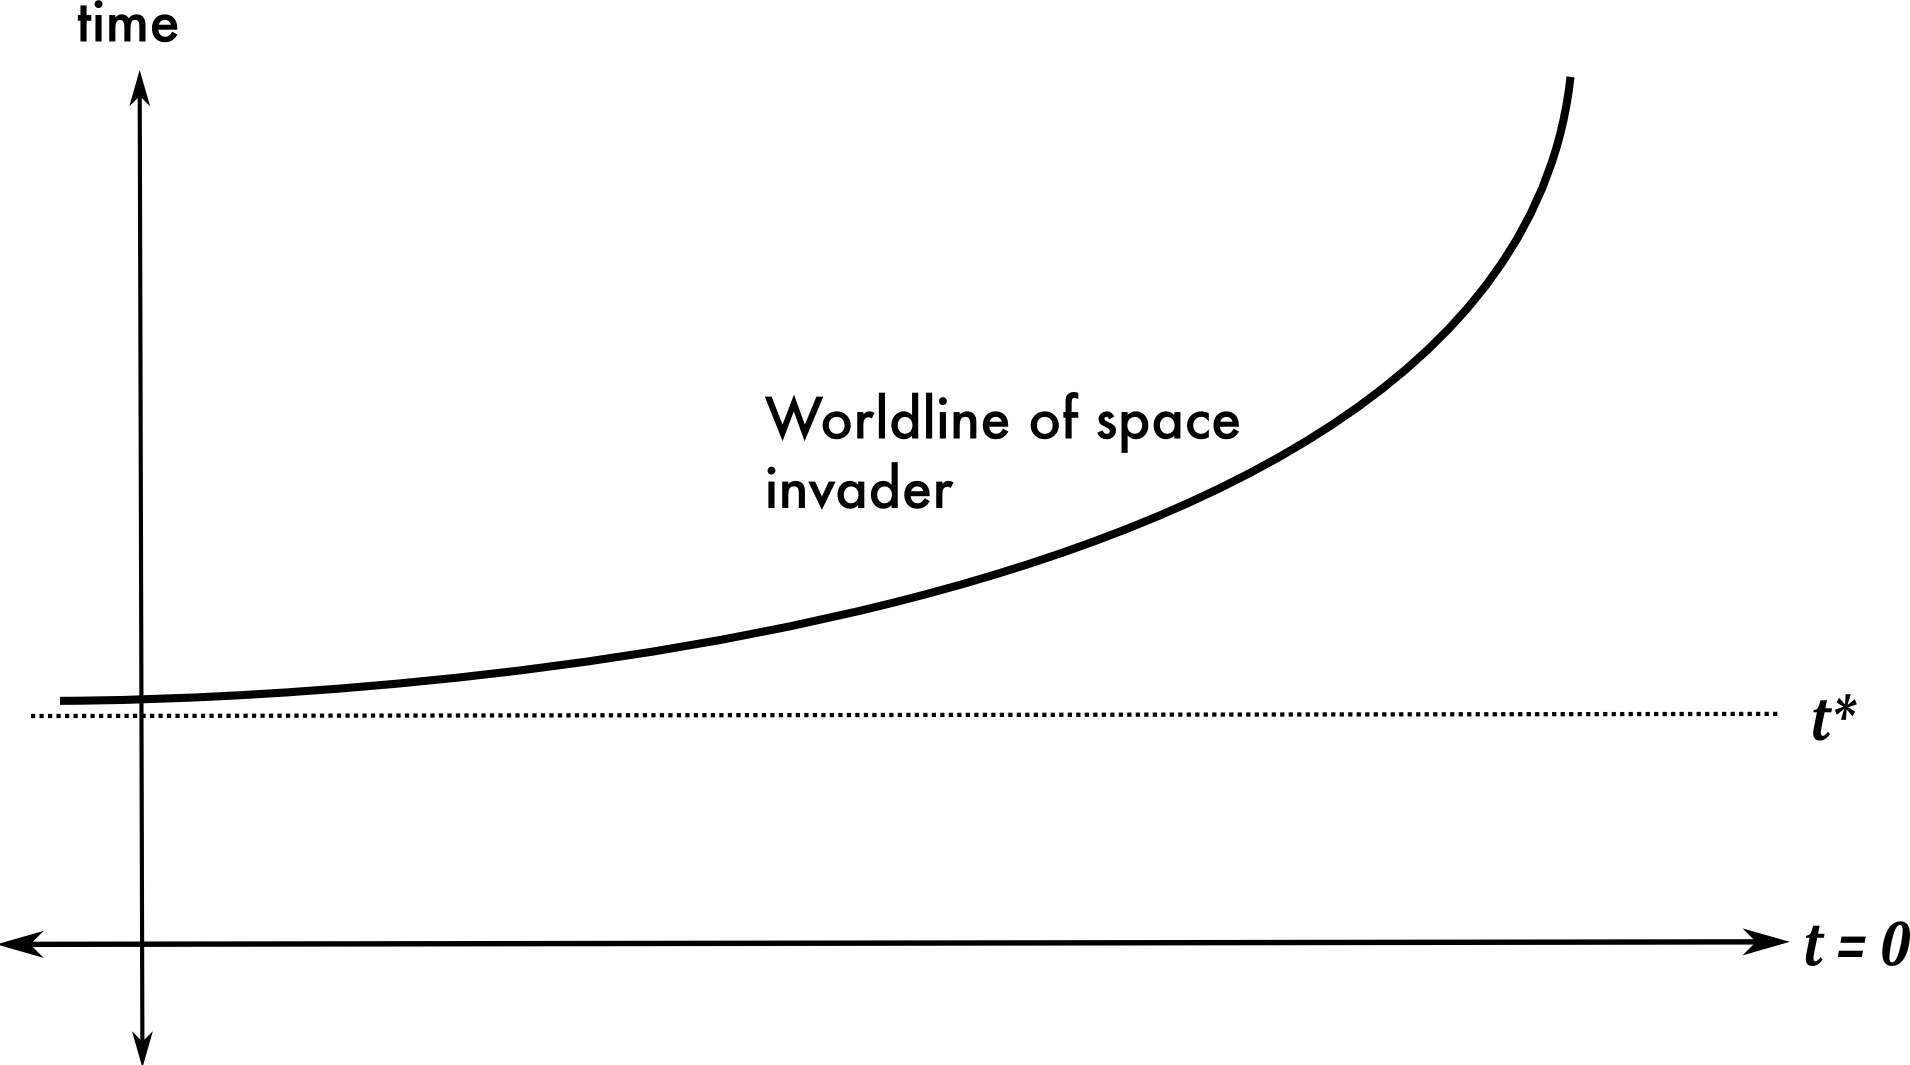
\includegraphics[scale=0.18]{space-invader.jpg}  
% \end{center}

% \vspace{10em}

% \begin{thebibliography}{999}
%     \bibitem{demon pic}
%       Maxwell's demon diagram.\\
%       https://commons.wikimedia.org/wiki/File:Maxwell\%27s\_demon.svg
%     \bibitem{infiniteaccel}
%       Off to Infinity in Finite Time.\\
%       \emph{Notices of the AMS}, Xia 1993.
% \end{thebibliography}
\end{document}